\newcommand{\nom}{Porte conteneur}
\newcommand{\sequence}{03}
\newcommand{\num}{04}
\newcommand{\type}{TD}
\newcommand{\descrip}{Résolution d'un problème en utilisant des méthodes algorithmiques}
\newcommand{\competences}{Alt-C3: Concevoir un algorithme répondant à un problème précisément posé}

\documentclass[10pt,a4paper]{article}
  \usepackage[french]{babel}
  \usepackage[utf8]{inputenc}
  \usepackage[T1]{fontenc}
  \usepackage{xcolor}
  \usepackage[]{graphicx}
  \usepackage{makeidx}
  \usepackage{textcomp}
  \usepackage{amsmath}
  \usepackage{amssymb}
  \usepackage{stmaryrd}
  \usepackage{fancyhdr}
  \usepackage{lettrine}
  \usepackage{calc}
  \usepackage{boxedminipage}
  \usepackage[french,onelanguage, boxruled,linesnumbered]{algorithm2e}
  \usepackage[colorlinks=false,pdftex]{hyperref}
  \usepackage{minted}
  \usepackage{url}
  %\usepackage[locale=FR]{siunitx}
  \usepackage{multicol}
  \makeindex

  %\graphicspath{{../Images/}}

  \renewcommand\listingscaption{Programme}

  %\renewcommand{\thechapter}{\Alph{chapter}}
  \renewcommand{\thesection}{\Roman{section}}
  %\newcommand{\inter}{\vspace{0.5cm}%
  %\noindent }
  %\newcommand{\unite}{\ \textrm}
  \newcommand{\ud}{\mathrm{d}}
  \newcommand{\vect}{\overrightarrow}
  %\newcommand{\ch}{\mathrm{ch}} % cosinus hyperbolique
  %\newcommand{\sh}{\mathrm{sh}} % sinus hyperbolique

  \textwidth 160mm
  \textheight 250mm
  \hoffset=-1.70cm
  \voffset=-1.5cm
  \parindent=0cm

  \pagestyle{fancy}
  \fancyhead[L]{\bfseries {\large PTSI -- Dorian}}
  \fancyhead[C]{\bfseries{{\type} \no \num}}
  \fancyhead[R]{\bfseries{\large Informatique}}
  \fancyfoot[C]{\thepage}
  \fancyfoot[L]{\footnotesize R. Costadoat, J. Genzmer, W. Robert}
  \fancyfoot[R]{\small \today}
  
  \definecolor{bg}{rgb}{0.5,0.5,0.5}
  \definecolor{danger}{RGB}{217,83,79}
  
  \fancypagestyle{correction}{%
  \fancyhf{}
  \lhead{\colorbox{danger}{\begin{minipage}{0.65\paperwidth} \textcolor{white}{\textbf{Correction}} \end{minipage}} }
  \rhead{
\includegraphics[width=2cm]{../../img/logo}}
  \lfoot{Juliette Genzmer, Willie Robert, Renaud Costadoat}
  \rfoot{\colorbox{danger}{\begin{minipage}{0.6\paperwidth} \begin{flushright}\textcolor{white}{\textbf{Correction}}\end{flushright} \end{minipage}} }}

  
  % macro Juliette
  
\usepackage{comment}   
\usepackage{amsthm}  
\theoremstyle{definition}
\newtheorem{exercice}{Exercice}
\newtheorem*{rappel}{Rappel}
\newtheorem*{remark}{Remarque}
\newtheorem*{defn}{Définition}
\newtheorem*{ppe}{Propriété}
\newtheorem{solution}{Solution}


\begin{document}

\section{Présentation de la problématique}

L'objectif de cet exercice est de générer la page de garde d'un document à partir de la consultation d'une base de données.

\begin{center}
 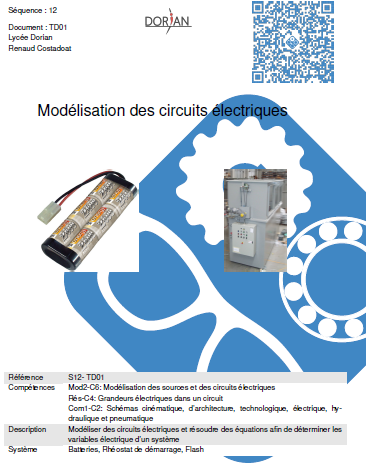
\includegraphics[width=0.6\linewidth]{img/img01}
\end{center}

L'objectif est de récupérer les infos suivantes afin de les insérer dans le document \LaTeX à générer:
\begin{itemize}
 \item Numéro de la séquence: $12$,
 \item Type de document: $C$, $TD$, $TP$, $KH$,
 \item Numéro du document: $01$, 
 \item Titre: 'Modélisation des circuits électriques',
 \item Compétences:
 	\begin{itemize}
  	\item \textit{Mod2-C6: Modélisation des sources et des circuits électriques,}
  	\item \textit{Rés-C4: Grandeurs électriques dans un circuit,}
  	\item \textit{Com1-C2: Schémas cinématique, d'architecture, technologique,	électrique, hydraulique et pneumatique.}
	\end{itemize}
 \item Description: \textit{Modéliser des circuits électriques et résoudre des équations afin de déterminer les
variables électrique d'un système}
 \item Systèmes : \textit{Batteries, Rhéostat de démarrage, Flash},
 \item Nom des fichiers des deux images qui vont apparaître sur la page de garde.
\end{itemize}

\section{Bases de données}

Des extraits des bases de données utiles sont données dans la suite.

~\

\begin{GrayBox}[0.85\textwidth]
\begin{verbatim}SELECT * FROM cours WHERE Sequence=12
\end{verbatim}
\end{GrayBox}

\begin{center}
\begin{tabular}{|p{1cm}|p{3cm}|p{1cm}|p{1cm}|p{1cm}|p{6cm}|}
\hline
\textbf{Id} & Nom & Seq & Num & Type & Description \\ \hline
13 & "Dipôles et sources électriques" & 12 & 1 & C & "Introduction à l'électronique de puissance, les dipôles, les sources de tension et de courant. Les associations de dipôles, les lois de l'électrocinétique." \\ \hline
18 & "Convertisseurs statiques" & 12 & 2 & C & "Les interrupteurs, la cellule de commutation, les hacheurs série, 2 quadrants, 4 quadrants et les onduleurs" \\ \hline
37 & "Modélisation des circuits électriques" & 12 & 1 & TD & "Modéliser des circuits électriques et résoudre des équations afin de déterminer les variables électrique d'un système" \\ \hline
44 & "Convertisseurs statiques" & 12 & 2 & TD & "Modélisation et mise en équation d'un convertisseur statique" \\ \hline
61 & "Modélisation des circuits électriques" & 12 & 1 & TP & "Modèles électriques. Résolution de la loi des noeuds. Loi des mailles." \\ \hline
76 & "Dipôles et sources électriques" & 12 & 1 & KH & "Introduction à l'électronique de puissance, les dipôles, les sources de tension et de courant. Les associations de dipôles, les lois de l'électrocinétique." \\ \hline
\end{tabular}
\end{center}

~\

\begin{GrayBox}[0.85\textwidth]
\begin{verbatim}SELECT * FROM systeme_util where Id>30 AND Id<40
\end{verbatim}
\end{GrayBox}

\begin{center}
\begin{tabular}{|p{0.5cm}|p{2cm}|p{2cm}|}
\hline
\textbf{Id} & Id\_systeme & Id\_cours \\ \hline
31 & 29 & 36 \\ \hline
32 & 30 & 36 \\ \hline
33 & 31 & 36 \\ \hline
34 & 32 & 37 \\ \hline
35 & 33 & 37 \\ \hline
36 & 34 & 37 \\ \hline
37 & 35 & 38 \\ \hline
38 & 36 & 39 \\ \hline
39 & 22 & 39 \\ \hline
\end{tabular}
\end{center}

~\

\begin{GrayBox}[0.85\textwidth]
\begin{verbatim}SELECT * FROM systemes WHERE Id>30 AND Id<36
\end{verbatim}
\end{GrayBox}

\begin{center}
\begin{tabular}{|p{1cm}|p{3cm}|p{6cm}|p{4cm}|}
\hline
Id & Systeme & Description & Img \\ \hline
31 & "Four industriel" & "Un four industriel permet électriquement de chauffer des pièces. Il peut avoir un très grand volume." & four\_industriel.jpg \\ \hline
32 & Batteries & "Une batterie d'accumulateurs, ou plus communément une batterie, est un ensemble d'accumulateurs électriques reliés entre eux de façon à créer un générateur électrique de tension et de capacité désirée. Ces accumulateurs sont parfois appelés éléments de la batterie ou cellule." & batteries.jpg \\ \hline
33 & "Rhéostat de démarrage" & "Un rhéostats est une résistance électrique réglable qui, intercalée dans un circuit, permet d'y modifier l'intensité du courant. Il est généralement constitué d'une résistance variable dimensionnée de manière à supporter l'intensité maximale du courant devant la traverser." & rheostat.jpg \\ \hline
34 & Flash & "Un flash photographique est un dispositif produisant une lumière intense pendant un très court laps de temps (environ 1/1000 de seconde), on l'utilise en photographie pour éclairer un sujet." & flash.jpg  \\ \hline
35 & "Variateur de vitesse" & "Un variateur de vitesse est un composant mécanique permettant de réduire une vitesse de rotation de manière continue." & variateur.jpg  \\ \hline
\end{tabular}
\end{center}

\newpage

\begin{GrayBox}[0.85\textwidth]
\begin{verbatim}SELECT * FROM competence_util WHERE Id>90 AND Id<100
\end{verbatim}
\end{GrayBox}

\begin{center}
\begin{tabular}{|p{0.5cm}|p{2cm}|p{4cm}|}
\hline
\textbf{Id} & Id\_cours & Id\_competence \\ \hline
92 & 35 & 15 \\ \hline
93 & 36 & 11 \\ \hline
94 & 36 & 42 \\ \hline
96 & 37 & 19 \\ \hline
97 & 37 & 41 \\ \hline
98 & 37 & 61 \\ \hline
99 & 38 & 13 \\ \hline
\end{tabular}
\end{center}

~\

\begin{GrayBox}[0.85\textwidth]
\begin{verbatim}SELECT * FROM competences WHERE Id>15 AND Id<20
\end{verbatim}
\end{GrayBox}

\begin{center}
\begin{tabular}{|p{1cm}|p{2cm}|p{3cm}|p{6cm}|p{2cm}|}
\hline
\textbf{Id} & Ref & Nom & Description & Semestre \\ \hline
16 & Mod2-C3 & "Systèmes linéaires discrets" & "Caractérisation des signaux à temps discret. Modélisation par équations aux différences, Modélisation de l'intégrateur par une somme discrète." & 3 \\ \hline
17 & Mod2-C4 & "Systèmes linéaires continus invariants asservis" & "Représentation par schéma bloc. Fonction de transfert en boucle ouverte et en boucle fermée, Classe d'un système" & 1 \\ \hline
18 & Mod2-C5 & "Systèmes à événements discrets" & "Modélisation des systèmes à événements discrets (fonctions logiques, tables de vérité, algorigrammes, graphe d'état), Modèles algorithmiques : structures algorithmiques élémentaires (boucles, conditions, transitions conditionnelles), Variables" & 2 \\ \hline
19 & Mod2-C6 & "Modélisation des sources et des circuits électriques" & "Modèle des sources parfaites continues et alternatives (générateur de tension ou de courant), Modèles de sources réelles par association de dipôles parfaits, Modélisation des circuits électriques par les lois de l'électrocinétique." & 2 \\ \hline
\end{tabular}
\end{center}

\newpage

\paragraph{Question 1:} Proposer une requête SQL visant à récupérer les informations suivantes:
\begin{itemize}
 \item Numéro de la séquence,
 \item Type de document,
 \item Numéro du document, 
 \item Titre,
 \item Compétences,
 \item Description,
 \item Systèmes.
\end{itemize}

\paragraph{Question 2:} Proposer une requête SQL permettant de ne récupérer que les nom des fichiers image de deux des systèmes utilisés dans le document.
\end{document}
